\subsection{5.3.3. 不同思考强度下的性能}\label{performance-across-reasoning-efforts}

图 9 报告了不同预算取值下的性能与平均响应长度。随着思考强度的提升，模型
产生越来越长的推理轨迹，推理密集型基准与软件工程任务上的准确率单调提升，
最大增益集中在低到中等的预算区间，继续增大则收益递减。尽管我们的 RL 只
涉及有限个强度档位，标量强度值仍能在特定区间内对响应长度实现灵活、可插值的
控制。这使实践者得以沿一条平滑的连续线权衡质量与延迟、token 成本：对延迟
敏感的应用可以在低强度档位下运行，只付出适度的准确率损失，而困难任务可以
调用高强度档位来恢复模型完整的推理能力。在我们的公开 API 服务中，我们
提供了三个预设强度档位，映射到这一标尺上：low、high 与 max 分别对应强度值
50、75 和 100。

\begin{figure}[htbp]
\centering
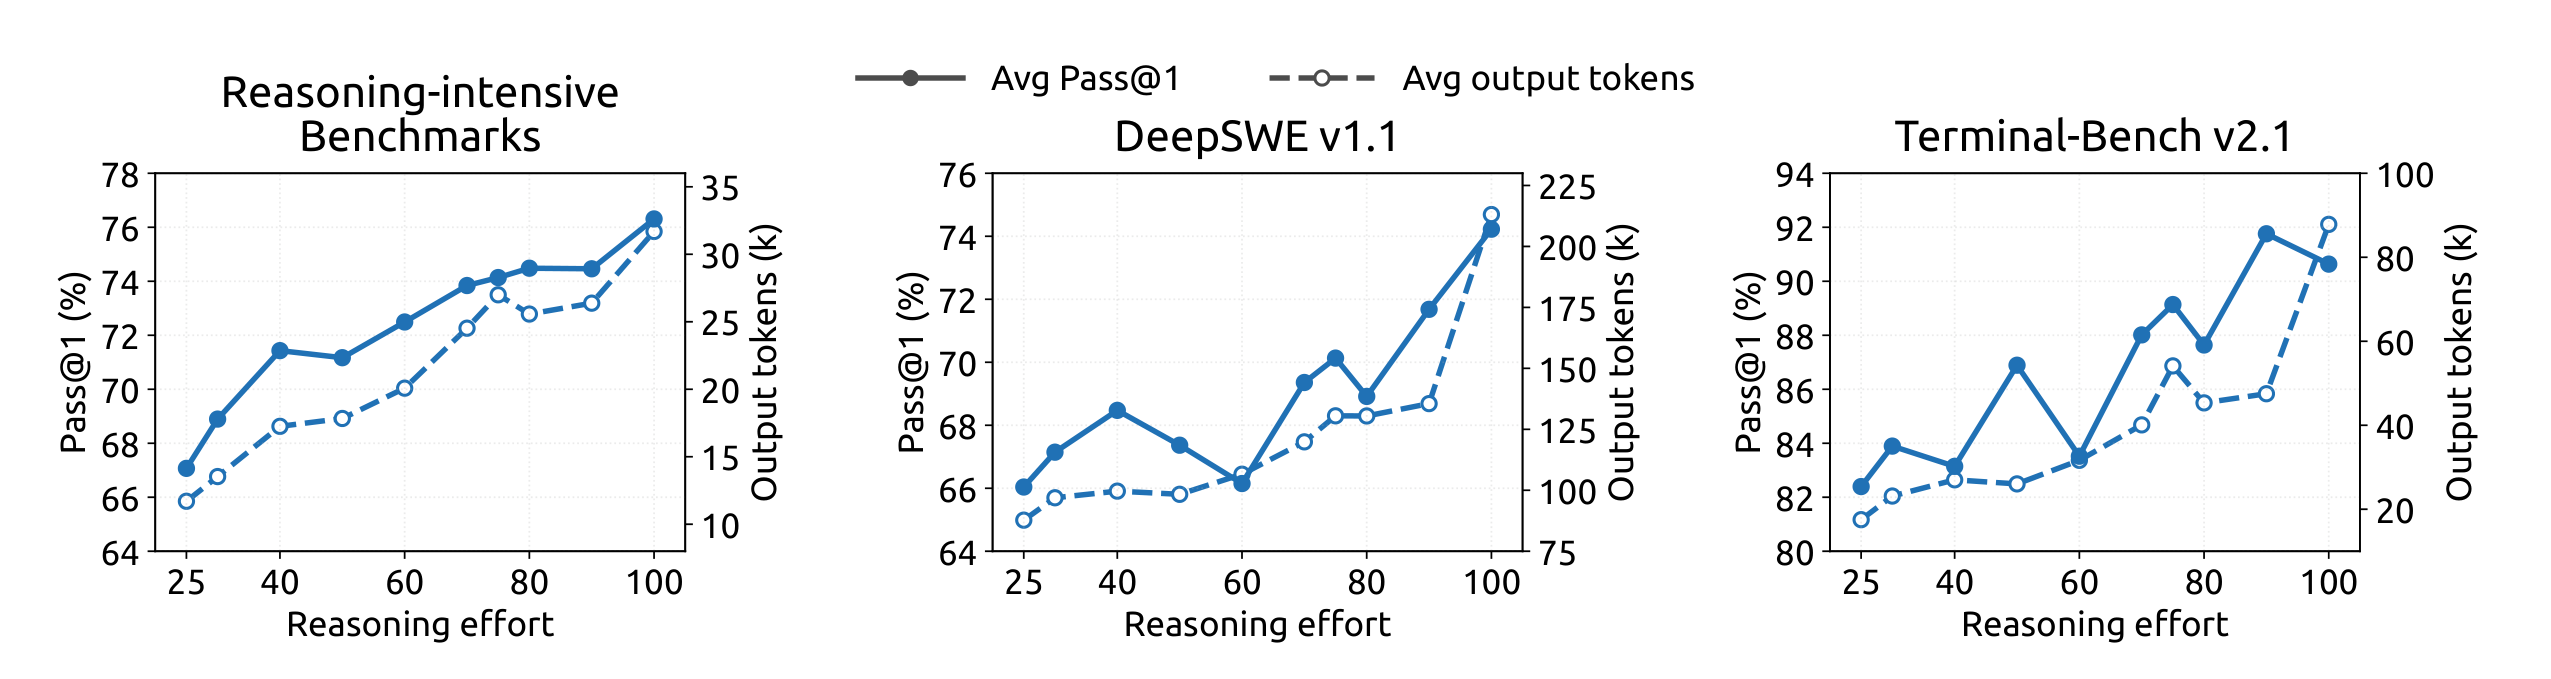
\includegraphics[width=\linewidth]{images_hi/fig09}
\caption{性能与输出长度随思考强度的变化。每个面板在思考强度取值从 25 变化到 100 时绘制 Pass@1（实线，左轴）和每条响应的平均输出 token 数（虚线，右轴）；推理密集型基准的结果为八个基准（AIME 2026、Apex 2025 Shortlist、GPQA Diamond、HLE、IMO-AnswerBench、LiveCodeBench、MathArena-Apex、SimpleQA-Verified）的平均值。DeepSWE v1.1 基于 mini-SWE 评估，Terminal-Bench v2.1 基于 DeepSeek Harness（Minimal）评估。}
\label{fig:9}
\end{figure}

\subsection{5.3.4. 不同智能体脚手架下的性能}\label{performance-across-agent-scaffolds}

在实践中，模型很少部署在某个单一的固定智能体框架中；不同脚手架在系统
提示词、工具定义、上下文管理策略与交互协议上各有差异，过度适配特定框架的
模型在换到另一个框架时可能大幅退化。为评估我们的模型对这种变化的鲁棒性，
我们的对比覆盖了来自六个脚手架族的八种配置：Claude Code（Anthropic, 2026）、
Codex（OpenAI, 2026）、OpenCode（Anomaly, 2026）、Pi（Zechner, 2026）、
mini-SWE（Yang et al., 2024），以及 Minimal、Standard、PTC 三种模式下的
DeepSeek Harness（DSH）（DeepSeek-AI, 2026a）。对每种脚手架，我们保持模型
checkpoint、解码配置与任务集完全相同，仅更换其外围框架，包括其原生系统
提示词、工具 schema 与轮次切换逻辑。表 4 报告了 DeepSWE v1.1 与
Terminal-Bench v2.1 上最大思考强度（100）下的性能。

模型的智能体能力能够很好地跨脚手架族迁移（这些脚手架族具有不同的提示词
与工具接口），而非依赖特定框架特有的约定。随着外围交互协议与工具抽象的
变化，其性能保持稳健，说明其智能体行为并未紧密耦合于单一脚手架设计。
这一鲁棒性与我们合成训练数据中环境、工具 schema 与交互格式的多样性
（第 5 节）一致，后者正是为鼓励跨智能体脚手架的泛化而设计。

表 4 \textbar{} 最大思考强度下各智能体脚手架的性能表现。

{\def\LTcaptype{none} % do not increment counter
\begin{longtable}[]{@{}lllllllll@{}}
\toprule\noalign{}
\endhead
\bottomrule\noalign{}
\endlastfoot
\multirow{2}{*}{基准（Metric）} & \multirow{2}{*}{Claude Code} & \multirow{2}{*}{Codex} & \multirow{2}{*}{OpenCode} & \multirow{2}{*}{Pi} & \multirow{2}{*}{mini-SWE} & \multicolumn{3}{l@{}}{%
DeepSeek Harness} \\
& & & & & & Minimal & Standard & PTC \\
DeepSWE v1.1 (Resolved) & 69.8 & 65.6 & 65.5 & 66.2 & 74.2 & 72.6 & 70.5
& 67.6 \\
Terminal-Bench v2.1 (Pass@1) & 88.0 & 84.1 & 85.0 & 86.1 & 90.3 & 90.6 &
85.8 & 85.8 \\
\end{longtable}
}

注：所有脚手架在 DeepSWE v1.1 上每任务使用 $N = 8$ 个样本，在
Terminal-Bench v2.1 上使用 $N = 3$ 个样本。两个基准的运行均使用 Linux
容器，temperature 1.0、top-p 0.95、1M-token 上下文窗口，以及每个智能体
max\_steps=500 轮的模型生成。Terminal-Bench v2.1 在无网络访问条件下评估。
我们评估了四个 Claude Code 版本，各版本结果及其平均值见附录表 5；本表报告
的是 v2.1.251。更多脚手架特定配置详见附录 B.1。

\subsection{5.3.5. 多智能体}\label{multi-agent}

为探索复杂任务上的多智能体协作，我们使用 DeepSeek Harness 的 Agent Team
模式对 DeepSeek-V4.1-Flash 进行了初步实验。

多智能体框架。我们在 Agent Team 模式下使用 DeepSeek Harness：主智能体
默认可以通过 spawn\_teammate 异步创建命名的、持久化的队友。每个队友都会
收到一个被委派的任务，并以两种模式之一启动：不带主智能体历史的 fresh 模式，
或带有主智能体已完成轮次一次性快照的 fork 模式。所有智能体共享同一个仓库
checkout，彼此的编辑立即可见。

智能体通过持久的对等邮箱通信。通过 send\_message 发送的消息会在下一次
步骤边界处送达正在运行的队友，为空闲队友开启新的一轮，或唤醒不活跃的队友。
在每位队友的任务生命周期内，主智能体用 list\_agents 监控运行时状态，并用
wait\_agent 等待状态、邮箱或共享任务的变化。任务归属、依赖关系与建议性写入
范围保存在共享任务板上（使用四个 team\_task\_* 工具，并在更新时做修订检查）。

当需要干预时，只有主智能体可以通过 interrupt\_agent 打断队友当前的一轮。
所需工作完成后，主智能体会审查并测试整合后的改动，生成最终响应。

训练。我们以结合任务表现、协作奖励与派生延迟惩罚的 RL 奖励来训练 Agent
Team 模式：协作奖励鼓励委派与智能体间通信，派生延迟惩罚促进高效协作。
派生延迟以有向无环图（DAG）表示执行事件及其协作依赖，按固定的 prefill/decode
速率由 token 数分配成本，再加上实测的工具执行时间，最后取关键路径的长度。
这既鼓励有用的并行，又惩罚不必要的串行工作与同步，同时降低对服务端批处理
与排队延迟的敏感度。

性能。我们从 ProgramBench（Yang et al., 2026）构造一个高置信度子集，仅保留
参考解在隐藏测试集上通过率至少达到 95\% 的任务。该过滤过程留下 172 个
``golden'' 任务。我们还评估了 FrontierSWE v2（Kondra et al., 2026）——
它是 FrontierSWE 更大、更有挑战性的后继版本，采用了显著改进的方法。我们
从当前公开任务中排除需要 GPU 访问的任务，构造出一个 no-GPU 子集。我们在
两个基准上、在明确的、每个 rollout 的挂钟截止时间下评估单智能体与多智能体
配置。这里报告的结果是初步的：我们用观测到的最强多智能体配置与可得的最强
单智能体基线进行比较。在 ProgramBench 上，每个任务最多运行三次 rollout，
对应每种配置 516 次计划的 rollout。我们报告 Almost@1，即得分至少达到 0.95
的单个 rollout 所占比例。在 FrontierSWE v2 上，我们报告 Mean@5。ProgramBench
的截止时间从 1 到 12 小时，而 FrontierSWE v2 在 1 到 20 小时的截止时间范围内
评估。在每个截止时间处，指标由截止时间到达时可得的所有输出计算。

如图 10 所示，在两个基准的每个截止时间处，多智能体配置都优于其单智能体
对应配置。在 ProgramBench 上，多智能体配置的 Almost@1 从 1 小时时的 13.59\%
升至 8 小时时的峰值 30.04\%，而单智能体配置为 12.79\% 与 20.39\%。在
FrontierSWE v2 上，多智能体配置的 Mean@5 从 1 小时时的 13.50\% 升至 20 小时
时的 32.90\%，而单智能体配置则从 10.50\% 升至 28.20\%。

\begin{figure}[htbp]
\centering
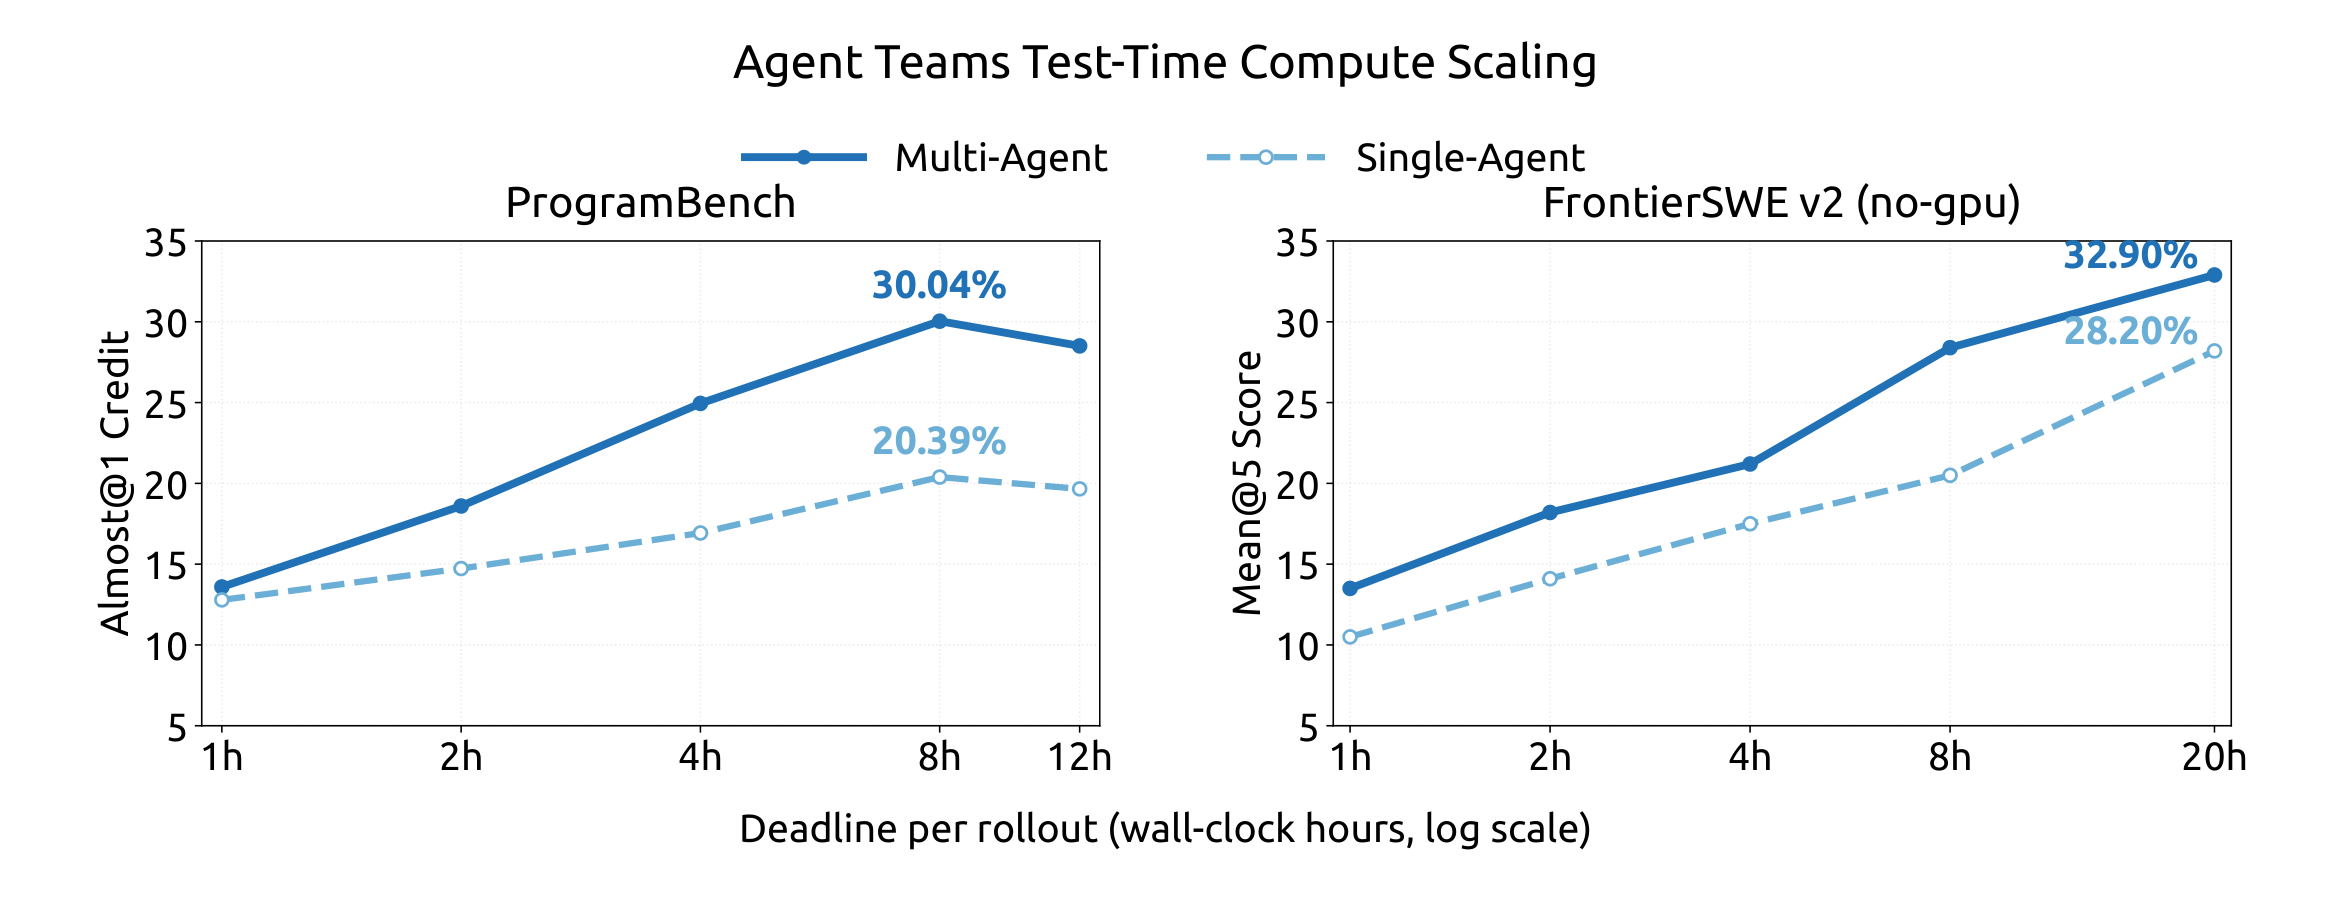
\includegraphics[width=\linewidth]{images_hi/fig10}
\caption{ProgramBench（Almost@1）与 FrontierSWE v2（Mean@5）上单智能体与多智能体配置的测试时计算扩展，作为每个 rollout 挂钟截止时间的函数。}
\label{fig:10}
\end{figure}